\chapter{应用层}

\begin{quote}
    \centering
    网络应用是计算机网络存在的理由
\end{quote}

\section{应用层协议原理}

    \emph{研发网络应用程序的核心是写出能够运行在不同的端系统和通过网络彼此通信的程序。}

    当研发新应用程序时,你需要编写将在多台端系统上运行的软件。重要的是,你不需要写在网络核心设备如路由器或链路层交换机上运行的软件。即使你要为网络核心设备写应用程序软件,你也不能做到这一点。网络核心设备并不在应用层上起作用,而仅在较低层起作用,特别是在网络层及下面层次起作用。这种基本设计,即将应用软件限制在端系统的方法,促进了大量的网络应用程序的迅速研发和部署。

\subsection{网络应用程序体系结构}

    当进行软件编码之前,应当对应用程序有一个宽泛的体系结构计划。从应用程序研发者的角度看,网络体系结构是固定的,并为应用程序提供了特定的服务集合。在另一方面,应用程序体系结构(application architecture)由应用程序研发者设计, 规定了如何在各种端系统上组织该应用程序。

\subsubsection{客户-服务器体系结构}

    在客户-服务器体系结构(client-server architecture)中,有一个总是打开的主机称为服务器,它服务于来自许多其他称为客户的主机的请求。\emph{值得注意的是利用客户-服务器体系结构,客户相互之间不直接通信}。

    客户-服务器体系结构的另一个特征是该服务器具有固定的、周知的地址,该地址称为IP地址。因为该服务器具有固定的、周知的地址,并且因为该服务器总是打开的,客户总是能够通过向该服务器的IP地 址发送分组来与其联系。

    在一个客户-服务器应用中,常常会出现一台单独的服务器主机跟不上它所有客户请求的情况。为此,配备大量主机的数据中心(data center)常被用于创建强大的虚拟服务器。

\subsubsection{P2P体系结构}

    在一个 P2P 体系结构(P2P architecture)中,对位于数据中心的专用服务器有最小的(或者没有)依赖。相反,应用程序在间断连接的主机对之间使用直接通信,这些主机对被称为对等方。因为这种对等方通信不必通过专门的服务器,该体系结构被称为对等方到对等方的。

    许多目前流行的、流量密集型应用都是P2P体系结构的。需要提及的是,某些应用具有混合的体系结构,它结合了客户-服务器和P2P的元素。

    P2P体系结构的最引人入胜的特性之一是它们的自扩展性(self-scalability)。例如, 在一个P2P文件共享应用中,尽管每个对等方都由于请求文件产生工作负载,但每个对等方通过向其他对等方分发文件也为系统增加服务能力。

\subsection{进程通信}

    用操作系统的术语来说,进行通信的实际上是进程(process)而不是程序。一个进程可以被认为是运行在端系统中的一个程序。当多个进程运行在相同的端系统上时,它们使用进程间通信机制相互通信。进程间通信的规则由端系统上的操作系统确定。

    此处,我们并不特别关注同一台主机上的进程间的通信,而关注运行在不同端系统(可能具有不同的操作系统)上的进程间的通信。

    在两个不同端系统上的进程,通过跨越计算机网络交换报文(message)而相互通信。发送进程生成并向网络中发送报文;接收进程接收这些报文并可能通过回送报文进行响应。

\subsubsection{客户和服务器进程}

    网络应用程序由成对的进程组成,这些进程通过网络相互发送报文。对每对通信进程, 我们通常将这两个进程之一标识为客户(client),而另一个进程标识为服务器(serve)。

    \emph{在一对进程之间的通信会话场景中,发起通信(即在该会话开始时发起与其他进程的联系)的进程被标识为客户,在会话开始时等待联系的进程是服务器}。

\subsubsection{进程与计算机网络之间的接口}

    多数应用程序是由通信进程对组成,每对中的两个进程互相发送报文。进程通过一个称为套接字(sock-et)的软件接口向网络发送报文和从网络接收报文。

    下图显示了两个经过因特网通信的进程之间的套接字通信(图中假定由该进程使用的下面运输层协议是因特网的TCP协议)。如该图所示,套接字是同一台主机内应用层与运输层之间的接口。由于该套接字是建立网络应用程序的可编程接口,因此套接字也称为应用程序和网络之间的应用程序编程接口(Application Programming Interface, API)。应用程序开发者可以控制套接字在应用层端的一切,但是对该套接字的运输层端几乎没有控制权。

\begin{figure}[!htbp]
    \centering
    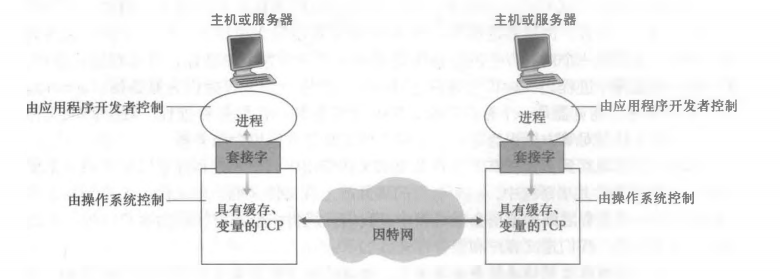
\includegraphics[width=0.6\textwidth]{image/chapter02/应用进程通信.png}
    \caption{应用程序间的套接字通信}
\end{figure}

    应用程序开发者对于运输层的控制仅限于:①选择运输层协议;②也许能设定几个运输层参数,如最大缓存和最大报文段长度等。

\subsubsection{进程寻址}

    在因特网中,主机由其IP地址(IP address)标识。此时,我们只要知道IP地址是一个32比特的量且它能够唯一地标识该主机就够了。除了知道报文发送目的地的主机地址外,发送进程还必须指定运行在接收主机上的接收进程(更具体地说,接收套接字)。因为一般而言一台主机能够运行许多网络应用, 这些信息是需要的。目的地端口号(port number)用于这个目的。

\subsection{可供应用程序使用的运输服务}

    包括因特网在内的很多网络提供了不止一种运输层协议。当开发一个应用时,必须选择一种可用的运输层协议。如何做出这种选择呢?最可能的方式是,通过研究这些可用的运输层协议所提供的服务,选择一个最能为你的应用需求提供恰当服务的协议。

    我们大体能够从四个方面对应用程序服务要求进行分类:可靠数据传输、吞吐量、定时和安全性。

\subsubsection{可靠数据传输}

    分组在计算机网络中可能丢失。在一些应用中,数据丢失可能会造成灾难性的后果。

    因此,为了支持这些应用,必须做一些工作以确保由应用程序的一端发送的数据正确、完全地交付给该应用程序的另一端。如果一个协议提供了这样的确保数据交付服务,就认为提供了可靠数据传输(reliable data transfer)。

    运输层协议能够潜在地向应用程序提供的一个重要服务是进程到进程的可靠数据传输。当一个运输协议提供这种服务时,发送进程只要将其数据传递进套接字,就可以完全相信该数据将能无差错地到达接收进程。

\subsubsection{吞吐量}

    在沿着一条网络路径上的两个进程之间的通信会话场景中,可用吞吐量就是发送进程能够向接收进程交付比特的速率。

    运输层协议能够以某种特定的速率提供确保的可用吞吐量。使用这种服务,该应用程序能够请求r比特/秒的确保吞吐量,并且该运输协议能够确保可用吞吐量总是为至少r比特/秒。这样的确保吞吐量的服务将对许多 应用程序有吸引力。

    具有吞吐量要求的应用程序被称为带宽敏感的应用(bandwidth-sensitive application)。带宽敏感的应用具有特定的吞吐量要求,而弹性应用(elastic application)能够根据当时可用的带宽或多或少地利用可供使用的吞吐量。

\subsubsection{定时}

    运输层协议也能提供定时保证。如同具有吞吐量保证那样,定时保证能够以多种形式实现。一个保证的例子如:发送方注入进套接字中的每个比特到达接收方的套接字不迟于100ms。

\subsubsection{安全性}
    
    运输协议能够为应用程序提供一种或多种安全性服务。这种服务将在发送和接收进程之间提供机密性,以防该数据以某种方式在这两个进程之间被观察到。运输协议还能提供除了机密性以外的其他安全性服务,包括数据完整性和端点鉴别。

\subsection{因特网提供的运输服务}

    我们已经考虑了计算机网络能够提供的通用运输服务。现在我们要更为具体地考察由因特网提供的运输服务类型。因特网(更一般的是TCP/IP网络)为应用程序提供两个运输层协议,即UDP和TCP。

\subsubsection{TCP服务}

    TCP服务模型包括面向连接服务和可靠数据传输服务。当某个应用程序调用TCP作为其运输协议时,该应用程序就能获得来自TCP的这两种服务。

\begin{table*}[!htbp]
    \begin{center}
        \caption{选择的网络应用的要求}
        \begin{tabular}{ | c | c | c | c | }
            \hline
            \textbf{应用} & \textbf{数据丢失} & \textbf{带宽} & \textbf{时间敏感} \\
            \hline
            文件传输 & 不能丢失 & 弹性 & 不 \\
            \hline
            电子邮件 & 不能丢失 & 弹性 & 不 \\
            \hline
            Web文档 & 不能丢失 & 弹性(几 kbps) & 不 \\
            \hline
            \multicolumn{1}{| c |}{\multirow{2}{*}{因特网电话/视频会议}} & \multicolumn{1}{c |}{\multirow{2}{*}{容忍丢失}} & 音频(几 kbps~1 Mbps) & \multicolumn{1}{c |}{\multirow{2}{*}{是,100ms}} \\
            \cline{3-3}
            \multicolumn{1}{| c |}{} & \multicolumn{1}{c |}{} & 视频(10 kbps~5 Mbps) & \multicolumn{1}{c |}{} \\
            \hline
            流式存储音频/视频 & 容忍丢失 & 同上 & 是,几秒 \\
            \hline
            交互式游戏 & 容忍丢失 & 几 kbps~10 kbps & 是,100ms \\
            \hline
            只能手机讯息 & 不能丢失 & 弹性 & 是和不是 \\
            \hline
        \end{tabular}
    \end{center}    
\end{table*}

\begin{itemize}
    \item [1)] 面向连接的服务
    \subitem 在应用层数据报文开始流动之前,TCP让客户和服务器互相交换运输层控制信息。这个所谓的握手过程提醒客户和服务器,让它们为大量分组 的到来做好准备。在握手阶段后,一个TCP连接(TCP connection)就在两个进程的套接字之间建立了。这条连接是全双工的,即连接双方的进程可以在此连接上同时进行报文收发。当应用程序结束报文发送时,必须拆除该连接。
    \item [2)] 可靠的数据传送服务
    \subitem 通信进程能够依靠TCP,无差错、按适当顺序交付所有发送的数据。当应用程序的一端将字节流传进套接字时,它能够依靠TCP将相同的 字节流交付给接收方的套接字,而没有字节的丢失和冗余。
    \item [3)] 拥塞控制机制
    \subitem 这种服务不一定能为通信进程带来直接好处,但能为 因特网带来整体好处。当发送方和接收方之间的网络出现拥塞时,TCP的拥塞控制机制会抑制发送进程(客户或服务器)。
\end{itemize}

\subsubsection{UDP服务}

    UDP是一种不提供不必要服务的轻量级运输协议,它仅提供最小服务。UDP是无连接的,因此在两个进程通信前没有握手过程。UDP协议提供一种不可靠数据传送服务,也就是说,当进程将一个报文发送进UDP套接字时,UDP协议并不保证该报文将到达接收进程。不仅如此,到达接收进程的报文也可能是乱序到达的

    UDP没有包括拥塞控制机制,所以UDP的发送端可以用它选定的任何速率向其下层(网络层)注入数据。(然而,值得注意的是实际端到端吞吐量可能小于该速率,这可能是因为中间链路的带宽受限或因为拥塞而造成的。)

\subsubsection{因特网运输协议所不提供的服务}

    在我们对TCP和UDP的简要描述中,明显地漏掉了对吞吐量或定时保证的讨论,即这些服务目前的因特网运输协议并没有提供。

    下表指出了一些流行的因特网应用所使用的运输协议。

\begin{table*}[!htbp]
    \begin{center}
        \caption{流行的因特网应用及其应用层协议与支撑的运输协议}
        \begin{tabular}{| c | c | c |}
            \hline
            \textbf{应用} & \textbf{应用层协议} & \textbf{支撑的运输协议} \\
            \hline
            电子邮件 & SMTP[ RFC 5321 ] & TCP \\
            \hline
            远程终端访问 & Telnet[ RFC 854 ] & TCP \\
            \hline
            Web & HTTP[ RFC 2616 ] & TCP \\
            \hline
            文件传输 & FTP[ RFC 959 ] & TCP \\
            \hline
            流式多媒体 & HTTP(如YouTube) & TCP \\
            \hline
            因特网电话 & SIP[ RFC 3261 ]、RTP[ RFC 3550 ] 或专用的(如Skype) & UDP或TCP \\
            \hline
        \end{tabular}
    \end{center}
\end{table*}

\subsection{应用层协议}

    应用层协议(application-layer protocol)定义了运行在不同端系统上的应用程序进程如何相互传递报文。特别是应用层协议定义了:

\begin{itemize}
    \item [1)] 交换的报文类型,例如请求报文和响应报文
    \item [2)] 各种报文类型的语法,如报文中的各个字段及这些字段是如何描述的
    \item [3)] 字段的语义,即这些字段中的信息的含义
    \item [4)] 确定一个进程何时以及如何发送报文,对报文进行响应的规则
\end{itemize}

    区分网络应用和应用层协议是很重要的。应用层协议只是网络应用的一部分(尽管从我们的角度看,它是应用非常重要的一部分)。

\section{Web和HTTP}

    Web是一个引起公众注意的因特网应用,它极大地改变了人们与工作环境内外交流的方式。它将因特网从只是很多数据网之一的地位提升为仅有的一个数据网。

\subsection{HTTP概况}

    Web的应用层协议是超文本传输协议(HyperText Transfer Protocol, HTTP),它是Web的核心。HTTP由两个程序实现:一个客户程序和一个服务器程序。客户程序和服务器程序运行在不同的端系统中,通过交换HTTP报文进行会话。HTTP定义了这些报文的结构以及客户和服务器进行报文交换的方式。

    Web页面(Webpage)(也叫文档)是由对象组成的。一个对象(object)只是一个文件,诸如一个HTML文件、一个JPEG图形、一个Java小程序或一个视频片段这样的文件,且它们可通过一个URL地址寻址。多数Web页面含有一个HTML基本文件(base HTML file)以及几个引用对象。

    HTML基本文件通过对象 的URL地址引用页面中的其他对象。每个URL地址由两部分组成:存放对象的服务器主机名和对象的路径名。Web服务器(Webserver)实现了HTTP的服务器端,它用于存储Web对象,每个对象由URL寻址。

    HTTP定义了Web客户向Web服务器请求Web页面的方式,以及服务器向客户传送Web页面的方式。如下图所示,客户与服务器交互的过程。

\begin{figure}[!htbp]
    \centering
    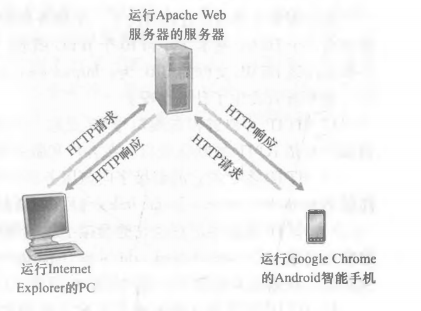
\includegraphics[width=0.6\textwidth]{image/chapter02/HTTP服务.png}
    \caption{HTTP请求-响应行为}
\end{figure}

    HTTP使用TCP作为它的支撑运输协议(而不是在UDP上运行)。HTTP客户首先发起一个与服务器的TCP连接。一旦连接建立,该浏览器和服务器进程就可以通过套接字接口访问TCP。

    客户向它的套接字接口发送HTTP请求报文并从它的套接字接口接收HTTP响应报文。类似地,服务器从它的套接字接口接收HTTP请求报文和向它的套接字接口发送HTTP响应报文。一旦客户向它的套接字接口发送了一个请求报文,该报文就脱离了客户控制并进入TCP的控制。

    这里我们看到了分层体系结构最大的优点,即\emph{HTTP协议不用担心数据丢失,也不关注TCP从网络的数据丢失和乱序故障中恢复的细节。那是TCP以及协议栈较低层协议的工作}。

    \emph{服务器向客户发送被请求的文件,而不存储任何关于该客户的状态信息。假如某个特定的客户在短短的几秒内两次请求同一个对象,服务器并不会因为刚刚为该客户提供了该对象就不再做出反应,而是重新发送该对象,就像服务器已经完 全忘记不久之前所做过的事一样。因为HTTP服务器并不保存关于客户的任何信息},所以我们说HTTP是一个无状态协议(stateless protocol)。

\subsection{非持续连接和持续连接}

    在许多因特网应用程序中,客户和服务器在一个相当长的时间范围内通信,其中客户发出一系列请求并且服务器对每个请求进行响应。依据应用程序以及该应用程序的使用方 式,这一系列请求可以以规则的间隔周期性地或者间断性地一个接一个发出。当这种客 户-服务器的交互是经TCP进行的。

    应用程序的研制者就需要做一个重要决定,即每个请求/响应对是经一个单独的TCP连接发送,还是所有的请求及其响应经相同的TCP连接发送呢?采用前一种方法,该应用程序被称为使用非持续连接(non-persistent connection);采用后一种方法,该应用程序被称为使用持续连接(persistent connection)。

\subsubsection{采用非持续连接的HTTP}

    我们看看在非持续连接情况下,从服务器向客户传送一个Web页面的步骤。假设该页面含有一个HTML基本文件和10个JPEG图形,并且这11个对象位于同一台服务器上。进 一步假设该 HTML 文件的 URL 为:http :〃www. someSchool. edu/someDepartment/home, indexo 我们看看发生了什么情况: 
    
\begin{itemize}
    \item [1)] HTTP客户进程在端口号80发起一个到服务器www.someSchool.edu的TCP连接,该端口号是HTTP的默认端口。在客户和服务器上分别有一个套接字与该连接相关联。
    \item [2)] HTTP客户经它的套接字向该服务器发送一个HTTP请求报文。请求报文中包含了路径名/someDepartment/home.index (后面我们会详细讨论HTTP报文)。 
    \item [3)] HTTP服务器进程经它的套接字接收该请求报文,从其存储器(RAM或磁盘)中 检索出对象 www.someSchool.edu/someDepartment/home.index,在一个 HTTP 响应报文中封装对象,并通过其套接字向客户发送响应报文。
    \item [4)] HTTP服务器进程通知TCP断开该TCP连接。(但是直到TCP确认客户已经完整地收到响应报文为止,它才会实际中断连接。)
    \item [5)] HTTP客户接收响应报文,TCP连接关闭。该报文指岀封装的对象是一个HTML文件,客户从响应报文中提取出该文件,检査该HTML文件,得到对10个JPEG图形的引用
    \item [6)] 对每个引用的JPEG图形对象重复前4个步骤
\end{itemize}

    上面的步骤举例说明了非持续连接的使用,其中每个TCP连接在服务器发送一个对象后关闭,即该连接并不为其他的对象而持续下来。值得注意的是每个TCP连接只传输一个请求报文和一个响应报文。因此在本例中,当用户请求该Web页面时,要产生11个TCP连接。

    我们给出往返时间(Round Trip Time, RTF)的定义,该时间是指一个短分组从客户到服务器然后再返回客户所花费的时间。RTT包括分组传播时延、分组在中间路由器和交换机上的排队时延以及分组处理时延。

\begin{figure}[!htbp]
    \centering
    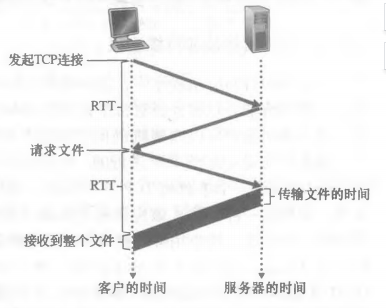
\includegraphics[width=0.6\textwidth]{image/chapter02/RTT.png}
    \caption{请求并接收一个HTML文件所需的时间估算}
\end{figure}

\subsubsection{采用持续连接的HTTP}

    非持续连接有一些缺点:
    
    第一,必须为每一个请求的对象建立和维护一个全新的连接。对于每个这样的连接,在客户和服务器中都要分配TCP的缓冲区和保持TCP变量,这给Web服务器带来了严重的负担,因为一台Web服务器可能同时服务于数以百计不同的客户的请求。

    第二,就像我们刚描述的那样,每一个对象经受两倍RTT的交付时延,即一个RTT用于创建TCP,另一个RTT用于请求和接收一个对象。

    在采用HTTP 1.1持续连接的情况下,服务器在发送响应后保持该TCP连接打开。在相同的客户与服务器之间,后续的请求和响应报文能够通过相同的连接进行传送。一般来说,如果一条连接经过一定时间间隔(一个可配置的超时间隔)仍未被使用,HTTP服务器就关闭该连接。HTTP的默认模式是使用带流水线的持续连接。

\subsection{HTTP报文格式}

HTTP 规范[ RFC 1945; RFC 2616; RFC 7540 ]包含了对HTTP报文格式的定义。HTTP报文有两种:请求报文和响应报文。

\subsubsection{HTTP请求报文}

\begin{lstlisting}[language=C++]
GET /somedir/page.html HTTP/1.1
Host: www.someschool.edu
Connection: close
User-agent: Mozilla/5.0
Accept-language: fr
\end{lstlisting}

    观察这个简单的请求报文,其中有五行信息,\emph{每一行的结尾都有一个结束符号(操作系统不同所对应的结束符号不同,在这里以$'\backslash{r}\backslash{n}'$为准)}。

    HTTP请求报文的第一行叫做请求行(request line),其后继的行叫做首部行(header line)。请求行有3个字段:方法字段、URL字段和HTTP版本字段。

    方法字段可以取几种不同的值,包括GET、POST、HEAD、PUT和DELETEO绝大部分的HTTP请求报文使用GET方法。当浏览器请求一个对象时,使用GET方法,在URL字段带有请求对象的标识。

    现在我们看看本例的首部行。首部行Host:www.someschool.edu指明了对象所在的主机。该首部行提供的信息是Web代理高速缓存所要求的。

    通过包含Connection: close首部行,该浏览器告诉服务器不要麻烦地使用持续连接,它要求服务器在发送完被请求的对象后就关闭这条连接。
    
    User-agent:首部行用来指明用户代理,即向服务器发送请求的浏览器的类型。这里浏览器类型是Mozilla/5.0,即Firefox浏览器。 这个首部行是有用的,因为服务器可以有效地为不同类型的用户代理实际发送相同对象的不同版本。(每个版本都由相同的URL寻址。)
    
    最后,Accept-language:首部行表示用户想得到该对象的法语版本(如果服务器中有这样的对象的话);否则,服务器应当发送它的默认版本。Accept-language:首部行仅是HTTP中可用的众多内容协商首部之一。

    接下来我们来看看请求报文的通用格式:

\begin{figure}[!htbp]
    \centering
    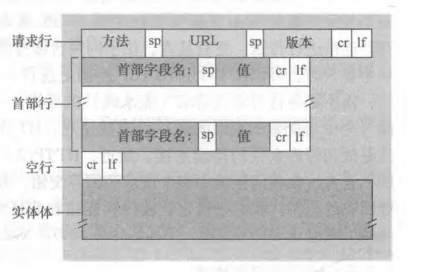
\includegraphics[width=0.6\textwidth]{image/chapter02/请求报文通用格式.png}
    \caption{HTTP请求报文的通用格式}
\end{figure}

    我们发现,在空行后有一个“实体体” (entity body)。\emph{使用GET方法时实体体为空,而使用POST方法时才使用该实体体}。当用户提交表单时,HTTP客户常常使用POST方法。如果方法字段的值为POST时, 则实体体中包含的就是用户在表单字段中的输入值。

    当然,值得注意的是,HTML表单经常使用GET方法,并在(表单字段中)所请求的URL中包括输入的数据。例如,一个表单使用GET方法,它有两个字段,分别填写的是"monkeys"和"bananas",这样,该URL结构为www.somesite.com/animalsearch?monkeys\&bananas。

    HEAD方法类似于GET方法。当服务器收到一个使用HEAD方法的请求时,将会用一个HTTP报文进行响应,但是并不返回请求对象。应用程序开发者常用HEAD方法进行调试跟踪。PUT方法常与Web发行工具联合使用,它允许用户上传对象到指定的Web服务器上指定的路径(目录)。PUT方法也被那些需要向Web服务器上传对象的应用程序使用。DELETE方法允许用户或者应用程序删除Web服务器上的对象。